\startfirstchapter{Introduction}
\label{chapter:introduction}

With the discovery of the Higgs boson in 2012 \cite{atlas_higgs_2012, cms_higgs_2012}, the final piece of the Standard Model fell into place. Developed during the latter half of the 20th century, the Standard Model describes all known particles and their interactions. The model has demonstrated remarkable predictive power, and can account for nearly all phenomena observed in particle physics detectors to date, with no firmly established deviations from its predictions. Yet, it is known to be incomplete. Among the observed phenomena that it fails to explain \cite{einstein_1920, neutrino_oscillations_1998, Canetti_2012} are multiple lines of astronomical observation that collectively point to the existence of a new form of non-luminous matter in the universe known as ``dark matter" (DM). 

While the nature of DM remains a mystery, the observational data strongly suggest that it will take the form of one or more new particles beyond the Standard Model. In addition to its gravitational interactions with massive particles, theoretical considerations 
%relating to the origin of DM in the universe 
give good reason to expect that the new particle(s) could experience additional, albeit weak, couplings to particles of the Standard Model by mechanisms yet to be determined. The study presented in this thesis is part of a multi-pronged international effort to search for evidence of particle DM by means of its non-gravitational interactions in particle physics experiments. In particular, this study probes new ground in the search for DM production in high-energy particle collisions at the Large Hadron Collider (LHC) at CERN. 

This chapter introduces the Standard Model, focusing on aspects that are particularly relevant to the presented search, and discusses the astronomical evidence for the existence of DM in the universe. It also introduces the range of experimental strategies that are currently employed to search for evidence of DM in particle physics detectors, and how this search fits into the wider DM search programme at the LHC. 
%in the context of existing searches for the Dark Higgs model, emphasizing the importance of facilitating re-interpretations to constrain other models that may be sensitive to the final state probed by the search. 

\section{Introduction to the Standard Model}

The Standard Model (SM) describes all known elementary particles and three of the four known forces by which they interact with one another - the strong, the electromagnetic (EM), and weak forces. The theory of general relativity \cite{einstein_1920}, which describes the gravitational force, has yet to be incorporated into the SM. 

The known particles, illustrated in Figure \ref{fig:standard_model} are divided into two classes known as ``fermions" and ``bosons" on the basis of an intrinsic form of angular momentum known as ``spin". Fermions carry spin \(\frac{1}{2}\), and bosons carry integer spin. 

The specific forces by which particles in the SM interact with one another are determined by the charge(s) that they carry. Particles that carry electric charge interact with other particles carrying this charge via the EM force. Similarly, particles that carry weak and colour charge interact via the weak and strong forces, respectively. 

Each fermion has a corresponding anti-particle with the same mass, but with opposite values of the charges it carries - for example, the electron \(e^-\) carries negative electric charge and its antiparticle, the positron \(e^+\), carries positive electric charge. 

\begin{figure}[H]
	\centering
	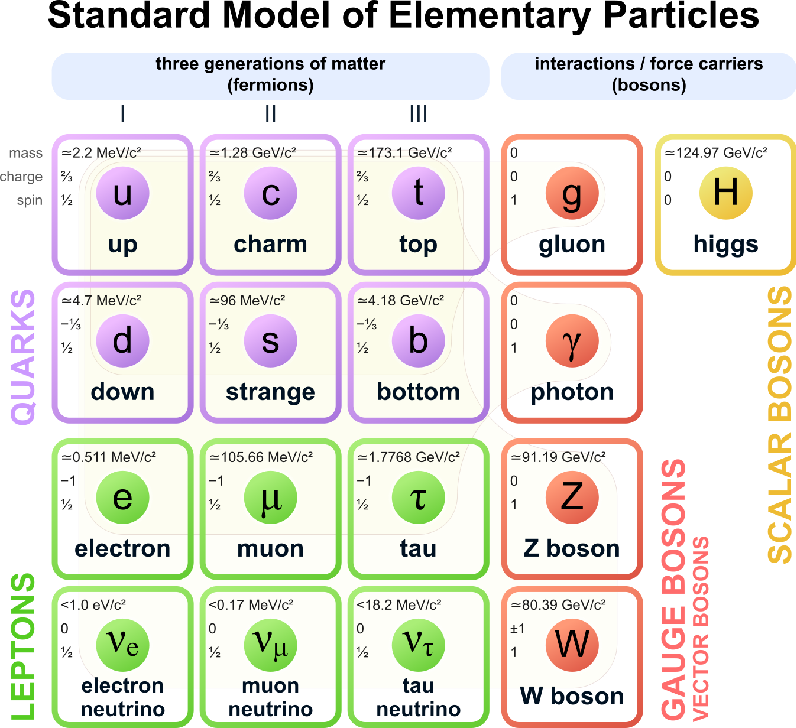
\includegraphics[width=0.7\textwidth]{Figures/1/StandardModel.pdf}
	\caption[]{Names and fundamental properties of particles in the Standard Model}
	\label{fig:standard_model}
\end{figure}

\subsection{Fermions}
\label{sec:fermions}

Fermions are further sub-divided into leptons and quarks, depending on the charges they carry, and hence by the forces with which they interact. There are three known generations of fermions, labelled I, II and III in Figure \ref{fig:standard_model}, each with significantly larger mass than the last. Each generation contains a pair of quarks and a pair of leptons, along with their associated antiparticles. The quark pair consists of one ``up-type" quark with positive electric charge and one ``down-type" with negative charge. The lepton pair consists of one charged lepton and one charge-neutral ``neutrino". 

Leptons carry electric charge and weak isospin, and as a result interact with one another and with other particles carrying these charges via the EM and weak forces, respectively.  

Like leptons, quarks also carry electric charge and weak isospin, and additionally carry colour charge. The colour charge allows quarks to interact via the strong force. As a result, quarks interact by all three forces described by the SM. Unlike charged leptons, which carry an electric charge of \(\pm1\), quarks carry fractional electric charge; up-type (down-type) quarks carry a charge of \(+\frac{2}{3}\) \(\big(-\frac{1}{3}\big)\).

Due to an effect known as ``colour confinement", quarks cannot exist as stable particles in isolation, and must instead combine with other quarks to form stable ``colour-neutral" states called ``hadrons". The two major forms of hadrons are ``mesons" formed by a quark-antiquark pair and ``baryons" formed by three quarks. Although the intrinsic strength (i.e. probability) with which particles couple via the strong interaction is 3 (14) orders of magnitude greater than via the EM (weak) interaction \cite{griffiths_2008}, the range of strong force interactions is limited by colour confinement to the approximate size of the proton (\(10^{-15}\)m). The LHC collides protons with sufficient energy to probe interactions between their constituent quarks and gluons at length scales smaller than the size of the proton. Due to the large strong force coupling at this scale, there is a relatively high probability that the interactions initiated by these collisions will proceed via the strong force compared with other forces. 
%As a result, the vast majority of decay products observed in the ATLAS detector are cascades of hadronic interactions in the calorimeter referred to as ``jets" \footnote{See Section \ref{sec:had_calo} for a more detailed discussion of jets in the hadronic calorimeter.} which are initiated by hadrons produced in the collisons.

\subsection{Bosons}

Bosons in the SM are divided into ``gauge bosons" and ``scalar bosons". The gauge bosons are spin 1 force carriers that mediate interactions between particles. The photon mediates EM interactions between electrically charged particles. The gluon mediates the strong interaction between quarks. Unlike charge-neutral photons, the gluon itself carries colour charge, which allows it to self-interact via the strong force. The weak force is mediated by three particles: the electrically neutral Z boson, and two W bosons (W$^\pm$) with opposite electric charges of $\pm$1. 

Scalar bosons are defined as spin 0 particles. There is only one scalar boson in the SM, namely the Higgs boson (or, simply, the ``Higgs") \cite{HiggsTheory1,HiggsTheory2,HiggsTheory3} . Particles in the SM acquire mass via their interaction with the Higgs field. As such, the Higgs only interacts with massive SM particles, which includes all particles except the photon and the gluon. The more massive the particle, the stronger its coupling with the Higgs. Neutrinos are a possible exception; there is at present no mechanism in the SM by which neutrinos could interact with the Higgs field, so the origin of their tiny masses remains an open question.  


\subsection{Collision and Decay Processes at Colliders}
\label{sec:col_decay_procs}

The high-energy counter-rotating proton beams at the LHC are brought into head-on collisions at four interaction points around the ring, each of which is surrounded by a detector\footnote{See Chapter \ref{chapter:lhc_atlas} for a detailed discussion of the LHC and the detectors that surround the four interaction points.}. At each interaction point, constituents of the colliding protons known as ``partons"\footnote{See Section \ref{sec:parton_model} for an introduction to the parton model.} can pair annihilate to form observable collision products via one or more ``virtual mediators"\footnote{See Section \ref{sec:virtual_particles} for a discussion of virtual particles.}, and the collision products are subsequently measured by the detector. 

Each process that describes a physically allowed mechanism by which partons may annihilate to form observable particles has a certain probability of taking place relative to other possible annihilation and production processes. The probability that a given process will take place is quantified by its ``cross section" \(\sigma\). The beam luminosity \(\mathcal{L}\) relates the rate of collisions \(\frac{dN}{dt}\) that proceed via a given process to the cross section of the process:

\begin{equation}
\frac{dN}{dt} = \mathcal{L}\sigma
\end{equation}

The luminosity can be integrated over a period of time \(t_1\) to \(t_2\), such that the total number of events expected to be produced via a process with cross section \(\sigma\) over the given period is related to the ``integrated luminosity" \(\mathcal{L}_\text{int}\) by:

\begin{equation}
\label{eq:integrated_lumi}
N = \sigma\int_{t_1}^{t_2}\mathcal{L}(t)dt = \sigma\mathcal{L}_\text{int}
\end{equation}

\subsection{Unstable Particles}

The lowest-mass ``first-generation" quarks and charged leptons located in column I in Figure \ref{fig:standard_model} are, along with neutrinos and the massless photons and gluons, the only stable particles in the SM. All other particles are unstable, and will decay to less-massive particles after they are produced. 

The decay of an unstable particle occurs randomly with respect to the time elapsed since the particle was produced, with the elapsed time governed by Poisson statistics. The probability \(P(t)\) that an unstable particle will have decayed after a time \(t\) has elapsed in its rest frame is given by the following cumulative exponential distribution:

\begin{equation}
\label{eq:particle_decay}
P(t) = 1-e^{-\frac{t}{\tau}} % = e^{-\Gamma t}
\end{equation}

\noindent where \(\tau\) is the mean lifetime of the particle.

%\noindent where the decay rate \(\Gamma\) is the inverse of the mean lifetime.  

\subsubsection{Unstable Resonance and the Breit-Wigner Formula}

Due to their finite lifetime, the Heisenberg uncertainty principle implies that unstable particles will not be produced with a well-defined mass, but rather with a mass distribution peaked at a central value \(m_0\). The probability density function \(p(m)\) associated with measuring an unstable particle with a mass \(m\) is given by the Breit-Wigner formula \cite{breit_wigner}:

\begin{equation}
\label{eq:breit_wigner}
p(m) \propto \frac{1}{(m-m_0)^2 + \frac{\Gamma_E^2}{4}}
\end{equation}

\noindent where \(\Gamma_E\) is the full width of the resonance peak. The lifetime of the unstable particle is related to the width of its Breit-Wigner resonance by \(\tau = \frac{\hbar}{\Gamma_E}\).

For unstable mediators produced in high-energy colliders that decay to a pair of detectable particles, the mediator mass can be reconstructed as the combined invariant mass\footnote{The invariant mass \(m\) of two particles with four-momenta \(p_1\) and \(p_2\) is in general given by: \(m^2 = p_1 \cdot p_2 = (E_1+E_2)^2 - (\mathbf{p}_1+\mathbf{p}_2)^2\)} of its measured decay products. Neglecting detector resolution effects, the cross section \(\sigma(m)\) associated with producing an unstable particle with a given reconstructed mass is expected to be proportional to its Breit-Wigner distribution: \(\sigma(m)\propto p(m)\). This results in a characteristic resonant peak in the reconstructed invariant mass distribution of the mediator's decay products, which can be used to identify the unstable mediator, and to measure its mass and lifetime.

\subsection{Feynman Diagrams}

The interaction mechanisms by which observable collision products are produced from the annihilation of two partons can be represented by Feynman diagrams, which are described in detail in Chapter 2 of Ref. \cite{griffiths_2008} and summarized here. As an example, the Feynman diagram for the Drell Yan process in which a \(q\bar{q}\) pair annihilate to form a lepton pair \(\ell\bar{\ell}\) via the exchange of a virtual photon (\(\gamma^{*}\))\footnote{The \(^{*}\) indicates that mass of the virtual particle may be off-shell (see discussion of virtual particles below).} or \(Z^{*}\) boson mediator is shown in Figure \ref{fig:drell_yan}. 

The particles involved in the interactions are represented as lines in a Feynman diagram, with different particle types represented by different line styles - fermions are generally represented by solid straight lines, and bosons (with the exception of gluons) are generally represented by wavy lines. Particle interactions are represented by vertices at which lines in the diagram intersect. The annihilation of a \(q\bar{q}\) pair to form the virtual \(\gamma^{*}/Z^{*}\) mediator is represented in Figure \ref{fig:drell_yan} by the vertex at which the \(q\) and \(\bar{q}\) fermion lines meet the \(\gamma^{*}/Z^{*}\) boson line, and the subsequent decay of the  \(\gamma^{*}/Z^{*}\) to \(\ell\bar{\ell}\) is represented by the vertex to the right at which the \(\gamma^{*}/Z^{*}\) line meets the \(\ell\) and \(\bar{\ell}\) lines. Note that time flows horizontally from left to right in Feynman diagrams, so the colliding \(q\bar{q}\) pair are shown on the left and the observable decay products \(\ell\bar{\ell}\) on the right.

\begin{figure}[h]
	\centering
%	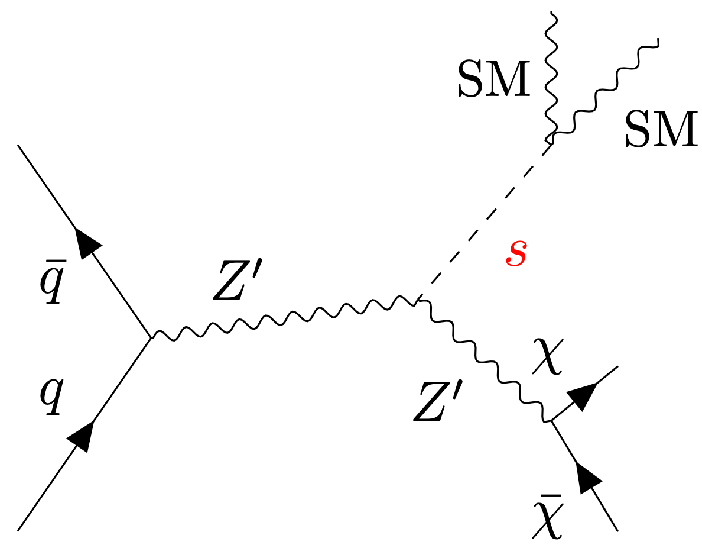
\includegraphics[width=0.95\textwidth]{Figures/2/Fey1.pdf}
		\begin{tikzpicture}
			\begin{feynman}

		 		\vertex (a1);
		 		\vertex at ($(a1) + (0cm, -3cm)$) (b1);
		 		\vertex at ($(a1) + (1cm, -1.5cm)$) (c1); %gamma/Z
		 		\vertex at ($(c1) + (2cm, 0cm)$) (c2); %gamma/Z
				\vertex at ($(c2) + (1cm, -1.5cm)$) (d1);
				\vertex at ($(c2) + (1cm, 1.5cm)$) (d2);

		 		\diagram* {
		 		  {[edges=fermion]
		 		    (b1) -- [edge label=\(q\)]( c1) -- [edge label=\(\bar{q}\)](a1),
				    (d1) -- [edge label=\(\bar{\ell}\)]( c2) -- [edge label=\(\bar{\ell}\)](d2),
		 		  },
		 		  (c1) -- [boson, edge label=\(\gamma^{*}/Z^{*}\)] (c2),
		 		};
		 	\end{feynman}
		 \end{tikzpicture}
	\caption{Feynman diagram for the Drell Yan process.}
	\label{fig:drell_yan}
\end{figure}

\subsubsection{Virtual Particles}
\label{sec:virtual_particles}

In general, ingoing and outgoing lines in a Feynman diagram represent real observable particles, and internal lines represent so-called virtual particles. Virtual particles are not observable, but are rather a representation of the mechanism involved with producing the observable final-state particles. Importantly, virtual particles can take on any mass needed to satisfy energy and momentum conservation at each interaction vertex.
% with which they are involved. 
% are not in general produced with the mass of their corresponding real particle, but can in principle take on whatever mass is needed to satisfy energy and momentum conservation at each interaction vertex that they are involved with. 

\subsubsection{Matrix Element}

%In order to study collision events measured by particle detectors at the LHC, it is important to calculate the rate at which the detector would be expected to measure collision events which proceed by different processes, such as the Drell-Yan process shown in Figure \ref{fig:drell_yan}. 

The cross section associated with a process of particle production from \(pp\) collisions at the LHC, such as the Drell-Yan process shown in Figure \ref{fig:drell_yan}, is in general proportional to an integral of the squared matrix element \(|\mathcal{M(\boldsymbol{x}, \boldsymbol{\alpha})}|^2\):

\begin{equation}
\label{eq:matrix_element}
\sigma \propto \int|\mathcal{M(\boldsymbol{x}, \boldsymbol{\alpha})}|^2 d\boldsymbol{x} 
\end{equation}

\noindent where the quantities \(\boldsymbol{x}\) describe the dynamics (masses, momenta, quantum numbers, etc.) of the incoming and outgoing observable particles, and \(\boldsymbol{\alpha}\) are terms that describe the internal structure of the process represented by the Feynman diagram, including the coupling constants that quantify the interaction strength of the particles involved at each interaction vertex and an integration over the possible dynamics of the virtual particles. 

\subsection{Mathematical Formulation of the Standard Model}
\label{sec:sm_math}

The SM is formulated mathematically as a quantum field theory, in which particles of the SM are represented as excitations of quantum fields. The mathematical formulation of the SM is presented in detail in standard texts \cite{griffiths_2008, SM_intro}, and briefly summarized in this section, with focus placed on aspects that are relevant to later discussions in this thesis.

\subsubsection{Lagrangian Densities}

As in classical field theories, the quantum fields of the SM and their interactions are powerfully described by the formalism of Lagrangian densities, which are functions of the quantum fields and their derivatives. For example, interactions between photons and electrically charged fermions are described in quantum electrodynamics (QED) by the following Lagrangian density term:

\begin{equation}
\label{eq:qed_interaction}
\mathcal{L}_\text{QED, interaction} = -q\psi^\dagger(x)\gamma^0\gamma^\mu\psi(x) A_\mu(x)
\end{equation}

\noindent where \(\psi(x)\), a function of the four spacetime coordinates represented by \(x\), is the quantum spinor field of the spin-\(\frac{1}{2}\) fermions in the SM. \(A_\mu(x)\) represents the vector field of the massless spin-1 photon and \(\gamma^\mu\) are the Dirac matrices \cite{griffiths_2008}. The index \(\mu\) runs over the four spacetime coordinates. The factor \(q\) represents the electric charge of the fermion involved in the interaction and its value\footnote{The electric charges of all fermions in the SM are as follows: \(\pm1\) for charged leptons, \(+\frac{2}{3}\) (\(-\frac{1}{3}\)) for up (down) type quarks and 0 for neutrinos.} determines the strength of the interaction. 

\subsubsection{Symmetries and Groups Theory Description}

Symmetries in the Lagrangian density function associated with each fundamental interaction are described in the language of group theory by classifying the fundamental interactions into gauge groups that describe their symmetries. For example, QED exhibits a symmetry under local phase transformations, described by the unitary local gauge group U(1). This means that the Lagrangian \(\mathcal{L}_\text{QED}\) is invariant under the multiplication of the fermion spinor \(\psi(x)\) by a unitary function \(U = e^{i\theta(x)}\) (unitarity implies that \(U^\dagger U=1\)),
%, which represents a local phase transformation 
where \(\theta(x)\) can be any function of the spacetime coordinates \(x\). It is found that this symmetry can be ensured by the inclusion of the vector field \(A_\mu(x)\) in the QED Lagrangian, which is identified with the physical photon. Because it ensures invariance under the U(1) gauge group, the vector field \(A_\mu(x)\) is referred to as a ``gauge field", and the corresponding boson (the photon) as a ``gauge boson". The symmetries in the SM are described by the direct product\footnote{General definitions in group theory can be found, for example, in Section 1.1 of Ref. \cite{costa2012symmetries}.} of the U(1)\(\times\)SU(2)\(\times\)SU(3) gauge groups. 

\subsubsection{Quantum Chromodynamics}

The theory of quantum chromodynamics (QCD), presented in standard texts such as Ref. \cite{qcd_2007}, describes the strong interactions mediated by gluons between particles with colour charge (quarks and gluons). Its symmetries are described by the SU(3) gauge group. The quarks are represented by a three-component vector of spinors: \(\psi_c = \{\psi_r, \psi_g, \psi_b\}\), where the subscripts refer to the three colours - red, green and blue - that constitute the charges of the strong interaction. The QCD Lagrangian (see eg. Eq. 10.88 in Ref. \cite{griffiths_2008}) is symmetric under a transformation of the vector of quark spinors \(\psi_c\) by a \(3\times3\) SU(3) matrix, which is unitary with determinant 1. The SU(3) symmetry is ensured by the inclusion of an eight-component set \(\boldsymbol{\boldsymbol{A}_\mu}\) of vector gauge fields in the QCD Lagrangian. The associated gauge bosons are identified as the eight physical gluons, each of which possesses a unique superposition of \({rgb}\) colour states \cite{griffiths_2008}.

\subsubsection{Electoweak Theory and the Higgs Mechanism}

The mathematical descriptions of the weak and EM forces are unified into a single ``electroweak" theory (for a review, see \cite{electroweak_2012}) whose symmetries are described by the SU(2)\(\times\)U(1) product of gauge groups. 

Developed in 1954, Yang-Mills theory \cite{yang_mills_1954} showed that a set of three vector gauge bosons, referred to as the ``isospin triplet" \(\boldsymbol{W}\) are needed to satisfy the SU(2) symmetry, and a fourth massless vector gauge boson \(B\) is needed to satisfy the U(1) symmetry. Despite satisfying the SU(2) symmetry of the weak interaction, the weak isospin triplet predicted by Yang-Mills theory falls short of fully describing the physical \(W^{\pm}\) and \(Z\) bosons that mediate the weak interaction, which are known to be massive \cite{pdg_2020}.

The U(1)\(\times\)SU(2)\(\times\)SU(3) symmetry of the SM Lagrangian does not admit mass terms of the form \(m_X^2X^\dagger X\), where X is an arbitrary field. Proposed in 1964, the ``Higgs mechanism" \cite{HiggsTheory1,HiggsTheory2,HiggsTheory3} provides a means of generating the masses of the physical \(W^\pm\) and \(Z\) bosons, as well as all other massive particles (with the exception of neutrinos), by adding the following term to the SM Lagrangian:

\begin{equation}
\label{eq:higgs_lagrangian}
\mathcal{L}_\text{Higgs} = (D^\mu H)^\dagger(D_\mu H) - V(H)
\end{equation}

\noindent where

\begin{equation}
H = \frac{1}{\sqrt{2}}
\begin{pmatrix}
0 \\
h+v
\end{pmatrix}
\end{equation}

 \(h(x)\) is interpreted as the scalar field of the physical Higgs boson, and \(v\) as the so-called ``vacuum expectation value". With \(H\) in this form, \(\mathcal{L}_\text{Higgs}\) is described by the U(1) symmetry group but not the SU(2) group, and is thus said to ``break" the electroweak symmetry SU(2)\(\times\)U(1) to the QED gauge symmetry U(1).

The covariant derivative \(D_\mu H\) in Eq. \ref{eq:higgs_lagrangian} takes the form:

\begin{equation}
\label{eq:D_muH}
D_\mu H = \big(\partial_\mu + i\frac{1}{2}g\sigma_k W^k_\mu+i\frac{1}{2}g'B_\mu\big)H
\end{equation}

\noindent where \(\sigma_k\) are the Pauli matrices, and \(g\) and \(g'\) are the coupling constants between the Higgs field and the \(\boldsymbol{W}\) and \(\boldsymbol{B}\) fields, respectively.

The Higgs potential \(V(H)\) takes the form:

\begin{equation}
V(H) = -\mu^2H^\dagger H + \lambda(H^\dagger H)^2
\end{equation}

\noindent where the second term describes quartic self-interactions of the Higgs field.

The emergence of the massive physical \(W^\pm\), \(Z\) bosons and the massless photon comes from the interactions of the electroweak \(\boldsymbol{W}\) and \(B\) fields with the Higgs field to produce ``mass" terms in the Lagrangian of the form \(m_X^2X^\dagger X\). This can be seen by expanding Equations \ref{eq:higgs_lagrangian} and  \ref{eq:D_muH}, considering only the terms involving the vacuum expectation value \(v\):

\begin{equation}
\label{eq:higgs_expanded}
\mathcal{L}_\text{Higgs} = \frac{v^2}{8}\Big[g^2\big((W^1_\mu)^2+(W_mu^2)^2\big) + (gW^3_\mu-g'B_\mu)^2\Big] + [...]
\end{equation}

With the physical vector boson fields and masses defined as:

\begin{equation}
\label{eq:physical_v_bosons}
\begin{split}
W^\pm_\mu & \equiv \frac{1}{2}(W_\mu^1 \mp W_\mu^2) \phantom{xxxxxxxxxlxx}\text{ with mass }\phantom{xxx} m_W=\frac{gv}{2} \\
Z_\mu & \equiv \frac{1}{\sqrt{g^2+g'^2}}(gW_\mu^3-g'B_\mu) \phantom{xxx}\text{ with mass }\phantom{xxx} m_Z = \frac{v}{2}\sqrt{g^2+g'^2} \\
A_\mu & \equiv \frac{1}{\sqrt{g^2+g'^2}}(g'W^3_\mu+gB_\mu) \phantom{xxx}\text{ with mass }\phantom{xxx} m_A = 0
\end{split}
\end{equation}

Inserting the definitions of the physical vector boson fields from Eq. \ref{eq:physical_v_bosons} back into Eq. \ref{eq:higgs_expanded}, it can be readily confirmed that Eq. \ref{eq:higgs_expanded} takes the form \(\mathcal{L}_\text{Higgs} = \big[(W^\pm)_\mu^\dagger(W^\pm)^\mu + Z_\mu^\dagger Z^\mu + A_\mu^\dagger A^\mu\big] + [...]\). Masses of fermions are likewise generated by so-called Yukawa couplings \cite{weinberg_1967} between the fermion and Higgs fields. The dark Higgs model used to optimize and interpret the DM search presented in this thesis postulates that DM, as well as any hypothetical new bosons that mediate its interactions with SM particles, would acquire their masses by means of their interaction with the dark Higgs field \(S\), as discussed in Chapter \ref{chapter:dh_model}. 


\section{Evidence for Dark Matter from Observational Astronomy}

Looking beyond the SM, many independent astronomical observations collectively provide compelling evidence for the presence and abundance of a new form of matter in the universe that is not directly observable because it neither emits nor absorbs light. Some of the earliest and clearest evidence for this so-called ``dark matter" (DM) came in 1978, when Rubin et al. \cite{Rubin_et_al} reported systematic anomalies in measured rotation speeds of spiral galaxies. In particular, distributions of the rotation speed as a function of the radial distance from the galactic centre differed in shape from what would be expected on the basis of the distribution of galactic mass measured from the observed luminosity profile. 

\begin{figure}[H]
	\centering
	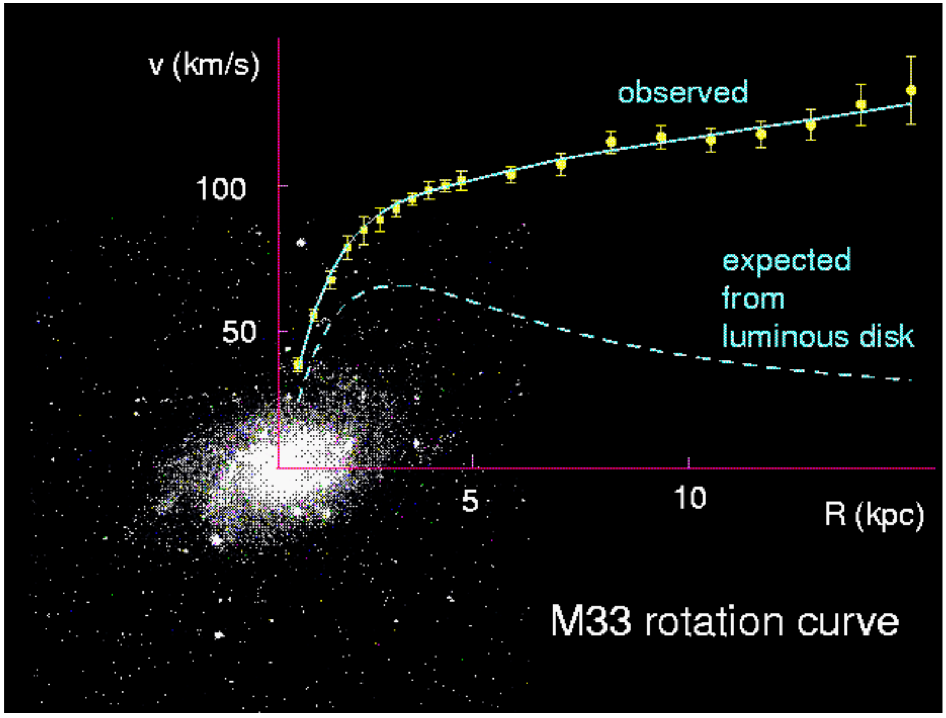
\includegraphics[width=0.6\textwidth]{Figures/1/m33_rotation.pdf}
	\caption[]{Observed rotation speed of the nearby dwarf galaxy M33, overlaid on an optical image of the galaxy. Yellow data points show observed rotational speed of the galaxy as a function of the radial distance from the galactic centre (in kpc). Dashed line shows the expected rotational speed on the basis of the calculated mass of the luminous stellar disk. Figure from \(\copyright\) \cite{m33_2000}.}
	\label{fig:m33_rotation}
\end{figure}

Spiral galaxies were known at the time to be comprised of a central spheroidal ``galaxy bulge" that contains the majority of luminous matter in the galaxy, in addition to a ``disk" extending out to larger radii from the galactic centre, within which the density of luminous matter falls off exponentially with radius. If one assumes that the distribution of mass in the spiral galaxy follows its luminosity profile, application of Newtonian gravitational mechanics\footnote{Rotation speeds of spiral galaxies are in general non-relativistic (typically \(v_\text{rot}/c<1\%\) \cite{rotn_curves_1995}). Since Newtonian gravitational mechanics represents an accurate approximation of general relativity in this macroscopic non-relativistic regime, it is generally assumed to provide an appropriate framework for the mathematical description of galactic rotation curves.} would predict the rotation speed to peak near the edge of the central galaxy bulge, as illustrated in the blue dashed line in Figure \ref{fig:m33_rotation} for the dwarf galaxy M33, and fall off at larger radii due to the exponentially decaying matter density of the disk. However, the observed galactic rotation speed, shown as yellow data points in Figure \ref{fig:m33_rotation}, is generally observed to continue increasing well beyond the luminous galactic bulge. These anomalies in galactic rotation curves, which have since been observed in hundreds of spiral galaxies \cite{rotn_curves_1995}, can be explained by postulating an additional source of non-luminous matter density in galaxies, DM, which extends well beyond the luminous bulge and provides the necessary gravitational potential to prevent the rotation speeds from falling off beyond the bulge.

In the years following the early reports by Rubin et al., modifications to the laws of Newtonian gravity at galactic scales \cite{mond_1983} were considered as an alternative to explain the anomalies without invoking the need for DM. However, while the proposed modifications to gravity were successful in describing the observed galactic rotation curves, numerous astronomical observations in other contexts have independently turned up results that indicate a need for DM in the universe, many of which cannot be easily explained by modifying Newtonian gravity. Additional evidence at galactic scales comes from significant differences between the spatial distributions of matter density, measured using gravitational lensing, and of luminous matter following collisions of galaxy clusters, such as the Bullet Cluster first identified in 1995 \cite{bullet_1995}, which indicate that the majority of the matter density in the colliding galaxies is non-luminous. Studies of the relative contribution to the masses of galaxy clusters from luminous matter using data from the Chandra X-ray observatory \cite{Chandra_2013} suggest that only 15-20\% of the mass composition of the galaxies studied is comprised of luminous matter, with DM comprising the remaining 80-85\%.
 
Because of their stability and EM interactions, protons and neutrons comprised of bound quarks, as well as their bound electrons - collectively known as ``baryonic matter" - comprise by mass the overwhelming majority of known luminous matter in the universe. The theory of Big Bang nucleosynthesis (BBN) (for a review, see Section 24 of \cite{pdg_2020}) predicts that the production of light nuclei - D, \(^2\)He, \(^4\)He, and \(^7\)Li - took place in the early universe following the Big Bang (reviewed in Ref.  \cite{uzan2016bigbang}), as the universe expanded and cooled sufficiently to allow their formation by means of nuclear fusion reactions. Importantly, BBN theory predicts that the abundances of these light nuclei in the universe were fixed during BBN, following which the rate of the nuclear fusion reactions became negligibly small due to the continued expansion and cooling of the universe. The theory also predicts that the relative abundances of the light nuclei are highly sensitive to the density of baryonic matter in the universe, which was fixed prior to their formation. Precision measurements of the abundances of light nuclei, interpreted in the context of BBN theory, indicate that baryonic matter constitutes approximately 5\% \cite{pdg_2020} of the energy density of the universe. Current measurements of anisotropies in the cosmic microwave background (CMB) \cite{cmb_1965} measured by the Planck collaboration \cite{Planck_2020}, interpreted in the context of the \(\Lambda\)CDM model of cosmology (for a review, see Section 25 of \cite{pdg_2020}), indicate that approximately 30\% of the energy density of the universe is comprised of matter, with the missing 25\% identified as non-baryonic DM. This result implies that \(~85\%\) of all matter in the universe is comprised of non-luminous DM, consistent with the findings discussed above from measurements of galaxy clusters.
in a process known as Big Bang nucleosynthesis (BBN)

\section{Dark Matter Composition Hypotheses}

The previous section presented a diverse range of astronomical observations that collectively point to the need for DM in the universe. While active research continues within the theoretical community (see, for example, Refs. \cite{mond_2012, mond_2021}) into the possibility of modifying the laws of gravitation at astronomical scales to explain these observations without the need for DM, there are significant theoretical challenges involved with designing modifications that can consistently explain the range of observational anomalies at scales ranging from individual galaxies to galaxy clusters, while simultaneously addressing the apparent need for DM at cosmological scales from the discrepancy between measurements of the baryonic mass density from BBN and the much larger total mass density inferred from anisotropies in the CMB. As a result, DM is widely considered the leading hypothesis to explain the full range of observational data.

While the astronomical observations provide a wealth of information regarding the composition of DM in the universe by means of its gravitational effects on visible matter, they provide relatively few clues as to what actually comprises the DM. Its abundance in the present day universe indicates that it must be stable on cosmological timescales (i.e. billions of years). The evidence from BBN and CMB anisotropies indicates that the DM must be non-baryonic. Its non-luminous nature further implies that it neither emits nor absorbs photons, and therefore has negligible or no charge under the EM force. Besides baryons, neutrinos - with their tiny but nonzero masses\footnote{Current constraints from cosmology place an upper limit on the sum of neutrino masses from all generations of 0.17 eV, \(~3\times10^6\) times smaller than the electron mass.} - represent the only other massive stable particles currently known to the SM, and satisfy the requirement of being electrically neutral. However, the possibility of neutrinos constituting any appreciable fraction of the DM was ruled out by studies published in the 1980's \cite{neutrino_dm}, which demonstrated that the large scale structure of the universe would differ significantly from what is observed today if the mass density of the universe were dominated by neutrinos due to their ultra-relativistic velocity. More generally, analysis of the measured anisotropies in the CMB measured by the Planck collaboration \cite{Planck_2020} is found to strongly favour the standard \(\Lambda\)CDM model in which the DM is predominantly comprised of ``cold" particles, so called because they travel at non-relativistic velocities.

With the stable particles of the SM ruled out, the current most widely accepted hypothesis is that DM is comprised of a new form of cold non-baryonic matter that is not currently described by the SM.

\subsection{Origin and Interactions of Particle Dark Matter}
\label{sec:dm_origins}

Despite the observable effects of its gravitational interactions at astronomical scales, the strength of gravitational couplings between massive particles is \(\sim30\) orders of magnitude weaker than any of the other three known forces \cite{griffiths_2008}. As a result, gravitational interactions between DM and SM particles are far too weak to be observable in particle detectors. Given that there have not yet been any conclusive indications of DM in particle detectors, it can be further deduced that any non-gravitational interactions between DM and particles of the SM are relatively weak compared with the strong, weak and EM couplings between SM particles. However, most theories that aim to describe the origin of the observed abundance of DM in the present day universe imply the existence of non-gravitational couplings between DM and SM particles, and in many cases predict that the couplings could be strong enough to be probed by modern particle detection methods. This produces a generic class of DM candidates known as weakly-interacting\footnote{The ``weak" interactions of the WIMP DM candidates are in general not necessarily associated with the weak force, but are simply too weak to have produced a measurable signature in particle detectors to date} massive particles (WIMPs). 
%The strength of the WIMP hypothesis has inspired worldwide efforts spanning several decades to design increasingly sensitive particle detectors and targeted studies to detect evidence of WIMPs. Such a detection would not only confirm the WIMP hypothesis,

A positive detection of WIMPs would not only confirm the hypothesis of particle DM, but would also allow physicists to begin to study its properties as a particle, and test theoretical extensions of the SM that incorporate particle DM.

\subsubsection{Dark Matter Origin from Thermal Freeze-out}

A review of the existing hypotheses for the origin of DM can be found in Section 27.3 of Ref. \cite{pdg_2020}. Of these, the so-called ``thermal freeze-out" scenario is a popular candidate, because it postulates that the observed DM density in the present day universe originated from the same process of thermal decoupling that produced the primordial abundances of light nuclei in the well-tested BBN scenario discussed earlier. The hypothesis postulates that in the very early universe, matter was sufficiently dense and energetic to establish thermal equilibrium between DM and SM particles due to interactions between DM and SM particles (so-called ``DM-SM interactions"). As the universe expanded and cooled, eventually the rate of DM-SM interactions became too low to maintain thermal equilibrium between the two species. At this point, known as ``thermal freeze-out", DM became decoupled from SM particles, thus fixing the relic abundance of DM observed in the present-day universe. 

For cold DM relics (\(v/c\lesssim0.1\) at the time of freeze-out), and assuming that the relic abundance is predominantly set by direct DM-SM interactions, analysis of the observed relic abundance of DM in the context of the thermal freeze-out hypothesis (see, for example, Section B of Ref. \cite{dm_xsec_2015}) implies that the cross section for SM-DM interactions should be \(\sigma_\text{SM-DM}\gtrsim1\) pb, comparable to typical cross sections for interactions mediated by the weak force. Searches for DM in particle detectors (for a review, see \cite{wimp_searches_2018}) have yet to turn up any hints of a DM candidate with interaction cross sections with the SM near the weak scale. However, the cross section constraint can be significantly relaxed by considering a scenario in which the relic abundance of DM is set not by direct interactions between the DM and the SM, but rather by interactions between DM and an unstable mediator, which subsequently decays to SM particles \cite{secluded_dm_2008}. The DM search presented in this thesis is interpreted in the context of such a scenario, wherein the unstable mediator is the Dark Higgs boson \cite{Duerr_2016,Duerr2017}.

\section{Dark Matter Search Strategies}

There are three complementary approaches used to search for particle DM by means of its non-gravitational interactions. Direct detection searches \cite{billard2021direct} aim to detect evidence of a recoil induced by elastic scattering between a DM particle in the galactic halo and a target particle in the detector. Indirect searches \cite{CIRELLI_2012, conrad} use observational data to search for evidence of particles produced by DM annihilation or decay in particular regions of the observable universe that are expected to have a high DM density. Collider searches \cite{DM_colliders}, of which the work in this thesis is an example, study the decay products from high-energy collisions of subatomic particles to search for an above-background excess of events that could be consistent with DM having been produced in some of the collisions.

\subsection{Direct Detection}

Direct detection searches operate in very low-background environments, typically in underground facilities such as SNOLAB (for a review, see Ref. \cite{Lawson_2013}), in order to minimize elastic scattering events in the detectors from non-DM sources such as cosmic rays and radioactivity, and detailed studies are performed to determine the expected rate of events from all possible background sources. As a result, a significant excess of elastic scattering events, particularly if observed in multiple direct detection experiments, would offer a clear signature of interactions with DM in the galactic halo. 

If no evidence of excess scattering events is found, experiments place upper bounds on DM-nucleon interaction cross section with a largely standard set of methods and assumptions (most notably the local DM density and the relative speed with which the DM passes through Earth) (see, for example, Ref. \cite{dd_results_standards_2021}), which facilitates comparison between different experiments. Figure \ref{fig:dd_limits} summarizes the current upper bounds on the spin-independent\footnote{Spin-dependent vs. spin-independent DM-nucleon interactions differ according to whether the coupling is sensitive to the spin state of the target nucleon \cite{billard2021direct}.} DM-nucleon interaction cross section from all direct detection searches. The searches probe down to many orders of magnitude below the weak scale (\(\sigma\sim10^{-36}\)cm\(^{-2}\)) over \(\sim4\) orders of magnitude of candidate DM masses. However, current direct detection strategies generally suffer practical limitations to the ranges of DM masses and interaction cross sections that can be probed. The lower bound on accessible DM masses is in general dictated by the signal to noise ratio of the detector, referred to as the ``noise wall", which is quite difficult to overcome. The range of accessible cross sections is also bounded from below for most direct detection experiments by the so-called ``solar neutrino floor", below which the measured event rate becomes dominated by the irreducible flux of solar neutrinos passing through the Earth. 

\begin{figure}[h]
	\centering
	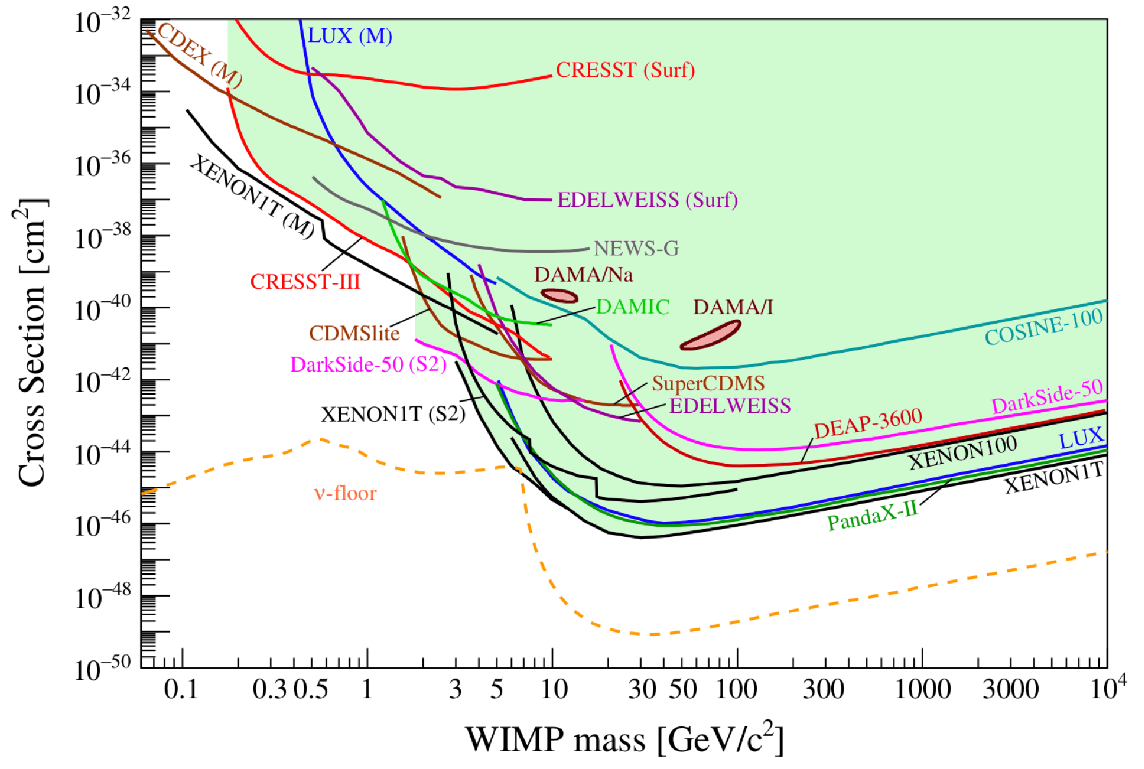
\includegraphics[width=0.7\textwidth]{Figures/1/dd_results.pdf}
	\caption[]{Summary of upper bounds from direct detection searches on the interaction cross section for spin-independent WIMP-nucleon scattering, over a range of hypothetical WIMP masses. Upper bounds from individual searches are shown as solid lines. Results labelled ``M" were obtained assuming the Migdal effect \cite{migdal_2018}. Shaded green region shows combined exclusion from all searches, excluding results obtained assuming the Migdal effect. Yellow dashed line shows the solar neutrino floor for a Ge target, computed using the assumptions and methodology presented in Refs. \cite{neutrino_floor_1, neutrino_floor_2}. Figure from \(\copyright\) \cite{billard2021direct}.}
	\label{fig:dd_limits}
\end{figure}

\subsection{Indirect Detection}

By searching for excesses of several potential DM annihilation products in observational data - gamma rays and charged leptons and antimatter - in addition to neutrinos, indirect detection searches (reviewed in Refs. \cite{conrad2014indirect, pdg_2020}) can avoid the limitation of the solar neutrino floor. Depending on the target species, these searches can also target a wider range of candidate DM masses compared with direct detection searches \cite{pdg_2020}. Due to the many potential processes that could produce the target particles in observational data - both within and beyond the SM - indirect searches generally contend with relatively large uncertainties associated with modelling the expected flux from these background sources. 
%Indirect searches generally probe \(\langle \sigma v \rangle\), where \(\sigma\) is the the DM-DM annihilation cross section, \(v\) is the velocity of the target DM relative to Earth, and the average represented by \(\langle\rangle\) is over the expected distribution of \(v\) as a function of the DM mass, for an assumed DM density in the target region. 

\subsection{Collider Searches}

Rather than searching for non-gravitational interactions of relic DM on Earth or in the observable universe, collider searches (for a review, see \cite{DM_colliders}) instead look for evidence of DM production from high-energy particle collisions. Like neutrinos, DM would be expected to pass invisibly through any detector surrounding the collision point due to its very low interaction cross section, producing a momentum imbalance transverse to the beam line referred to as \met\footnote{See Section \ref{sec:met} for a detailed introduction to missing transverse momentum in the ATLAS detector.}. An excess of collision events with large final-state \met above the rate expected from SM processes with final-state neutrinos would be consistent with the production of DM in the high-energy collisions. Given that other hypothetical new physics processes (see, for example, Refs. \cite{add_1998, dark_energy_lhc}) could also produce an excess of high-\met events from non-DM sources, any such findings would benefit from corroborating DM detections in direct and/or indirect detection experiments.

Despite operating in a very high background environment, collider searches offer numerous advantages that allow them to complement and potentially extend the reach of direct and indirect searches. First, the detectors used by particle colliders are often designed to measure all final-state particles produced by the collisions and their kinematic information with high precision. This detailed final-state information allows DM searches to target specific final-state topologies, which can lead to substantial reductions in SM background processes and considerably enhance the sensitivity to hypothetical DM production processes that predict events with the targeted topology. Second, by targeting DM produced in the collisions and adopting a search strategy that does not require the DM to interact with the detector, collider searches are insensitive to the neutrino floor that will challenge the sensitivity of next-generation direct detection searches. Third, while the range of DM masses is bound from above by the centre of maximum centre-of-mass energy of the particle collisions (\(\sim\)TeV for proton-proton collisions at the LHC), collider searches do not suffer the noise wall that limits the sensitivity of direct detection searches below \(\sim1~\GeV\) (see Figure \ref{fig:dd_limits}).

Event if particle DM is first discovered in a non-collider experiment, the detailed final-state information available in the particle collision data will enable detailed measurements of its properties and interactions, provided that it can be produced at colliders.

\subsection{Searching for Dark Matter at Particle Accelerators}

\subsubsection{Collider Search Approaches}

The concept of searching for evidence of DM production in high-energy particle collisions is currently being pursued by numerous collaborations. The particular energy scales and detector technologies available to each experiment can be exploited to target specific mass ranges and possible DM production mechanisms, thus allowing for a rich programme of complementary searches.

The proton-proton collision experiments at the Large Hadron Collider (LHC)\footnote{See Section \ref{chapter:lhc_atlas} for a general introduction to the LHC and its major detectors.} \cite{lhc_machine} - ATLAS \cite{atlas}, CMS \cite{cms} and LHCb \cite{LHCb} - benefit from the world-leading 13 TeV centre of mass energy of the \(pp\) collisions to probe models with massive mediators (\(m_\text{med}\) up to a few TeV) of the DM-SM interactions that could be produced in the collisions. The hermetic\footnote{Hermetic detectors, of which ATLAS and CMS are examples, are designed to detect all SM decay products from a collision with the exception of neutrinos.} coverage and precise event reconstruction available with the ATLAS and CMS general-purpose detectors make it possible to probe a wide range of hypothetical DM production models and final-state signatures, typically targeting DM candidates with masses in the \(\sim\)GeV-TeV range (see Ref. \cite{Trevisani:2018psx} for a review of DM searches performed with the ATLAS and CMS detectors). Meanwhile, DM searches at LHCb (for a review, see \cite{mombacher2021dark}) take advantage of the detector's excellent forward-angle coverage and vertex resolution to target signatures with lower-mass DM (\(\sim\)MeV-GeV) and displaced vertices.

In addition to proton-proton collisions at the LHC, production of DM in electron-positron \(e^+e^-\) collisions has been probed with the BABAR experiment \cite{babar_2002} at the Stanford Linear Accelerator Centre (SLAC), as well as the Belle experiment \cite{belle_detector_2002} and its recent Belle II upgrade \cite{belle_II_2018} at the SuperKEKB collider \cite{superkekb_2018}. With a 10.6 GeV centre of mass collision energy, the Belle II experiment is particularly well suited to study DM with masses in the range of a few MeV to 10 GeV. Searches at \(e^+e^-\) colliders benefit in precision both from the well-defined initial state afforded by colliding fundamental particles, and from the vastly reduced background of QCD activity\footnote{See Section \ref{sec:trigger} for a more detailed discussion of the QCD background in the context of the ATLAS triggering system.} in the final state compared with \(pp\) collision events. Searches performed with early Belle II data, reviewed in Ref. \cite{Campajola_2021}, are already showing promising sensitivity to a number of low-mass DM candidates, with significant sensitivity improvements expected as more data is collected in the coming years.

The most direct way to search for DM at \(pp\) and \(e^+e^-\) collider searches is to look for evidence of the so-called ``\met+X" events introduced above, in which the DM is produced along with detectable SM particles, thus producing a signature of SM particles recoiling against \met in the final state. An alternative approach, known as a ``resonance search", is to search for evidence of the production of new massive mediators that could potentially mediate DM-SM interactions by looking for resonant peaks in the invariant mass distribution of one or more pairs of final-state particles. Such a peak, if not associated with any known SM mediators, would be indicative of the production and subsequent decay of a new massive mediator to a pair of SM particles.

DM in the \(\sim\)MeV-GeV mass range can also be probed with competitive sensitivity at fixed-target experiments in which a beam of energetic electrons or protons is directed at a fixed target, and downstream detectors search for evidence of DM produced from the electron-nucleon or proton-nucleon collisions. A variety of approaches are employed by different experiments to search for signatures of DM production. Some searches re-purpose neutrino detectors, such as MiniBooNE \cite{miniboone_2018} and NOvA \cite{nova_2017} at Fermilab, to directly detect any DM that may be produced in the collisions by means of DM-nucleon or DM-electron collisions with the detector material, placing additional shielding between the fixed target and the detector to reduce the background flux of neutrinos. Others such as NA64 \cite{na64_2019} at CERN employ a fully hermetic detector to search for a \met+X signature of DM in the downstream collision products.

\subsubsection{Models of DM Production}

Models of DM production in colliders can range in complexity from an effective field theory (EFT), where the DM production mechanism is completely unspecified, to a complete model such as supersymmetry \cite{susy_dm}, which predicts viable DM candidates as part of a hypothesized extension to the SM designed to address a range of phenomena unexplained by the SM. 

%The EFT approach treats the production of DM from colliding partons as a contact interaction, with the production rate determined by a single parameter \cite{DM_colliders}. As long as a measurable SM particle is also produced in the interaction (eg. a gluon radiating from one of the colliding quarks, as in Figure \ref{fig:eft_simplified_model}), the EFT framework can be applied to any mono-X signature at the LHC, where a SM particle X is measured along with missing transverse momentum in the detector. This makes the framework generally usable in terms of motivating and providing a theoretical framework to interpret a range of generic search channels that can be readily selected for in LHC collision data. However, the EFT framework relies on the assumption that the the mediator(s) of the interaction is (are) much more massive than the scale of momentum transfer in the interaction \cite{DM_colliders, beyond_eft}. If this assumption is inaccurate, the EFT framework becomes invalid, and a more complete model is needed to specify additional details of the process leading to DM pair production. 

\begin{figure}[h]
	\centering
	\begin{minipage}[b]{0.45\textwidth}
	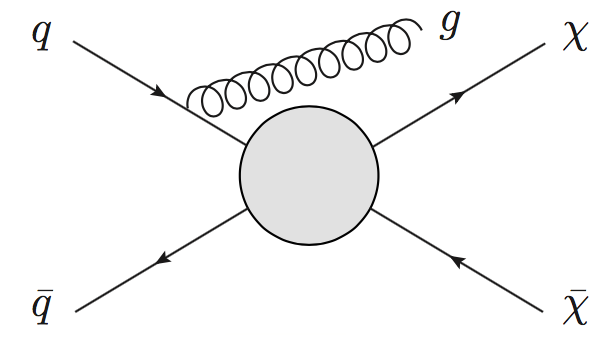
\includegraphics[width=0.9\textwidth]{Figures/1/EFT_Signature.png}
	\end{minipage}
	\begin{minipage}[b]{0.45\textwidth}
	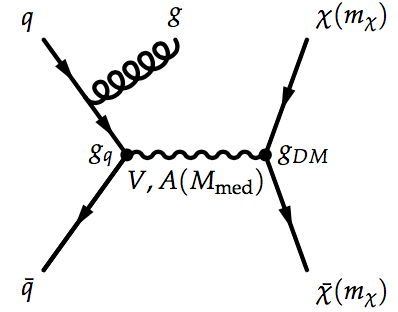
\includegraphics[width=0.8\textwidth]{Figures/1/simplified_model.png}
	\end{minipage}
	\caption[]{Left: \met+jets process in the EFT framework (source: \cite{beyond_eft}). Right: \met+jets process in a simplified model framework, where the pair production of DM occurs via a new vector or axial-vector ($V$, $A$) mediator of mass $M_\text{med}$, which couples to quarks and DM with coupling constants g$_q$ and g$_\text{DM}$, respectively (source: \cite{dm_forum})}.
	\label{fig:eft_simplified_model}
\end{figure}

In principle, complete theories of physics beyond the SM, such as the minimal supersymmetric SM (MSSM) (for a review, see \cite{mssm}) can offer theoretically motivated and experimentally accessible models that specify the details of candidate processes by which the colliding partons may annihilate to produce DM. However, these theories tend to be quite complex, with many free parameters - over 100 in the case of MSSM \cite{DM_colliders} - most of which need to be fixed to generate a reasonably testable model. Relying on complete theories alone to guide experimental signatures may run the risk of missing important parameter space of new physics for which a complete theory has not yet been developed. 

Simplified models, widely used in recent and ongoing DM searches at the LHC, are designed to bridge the gap between EFT and complete theories. They provide a ``first-order" description of theoretically motivated new physics scenarios that could be accessible at collider energies. They provide guidance for experimental searches without fully specifying the details of any additional new physics at energies above the collider scale that would be needed for a complete theory \cite{DM_colliders}. In terms of DM production at the LHC, one or more new ``portal mediators" associated with new physics scenarios may be considered, which allow for mixing between SM particles and DM. The process by which the mixing occurs is represented with a tree-level diagram whose experimental signature would be accessible at LHC energies, such as the diagram shown in Figure \ref{fig:eft_simplified_model}, which represents a DM benchmark model featured in the 2015 report of the ATLAS/CMS Dark Matter Forum \cite{dm_forum}. 

Many simplified models predict the so-called \met+X final-state signature discussed above, in which the DM is produced in association with detectable SM particles (X). Depending on the details of the hypothesized DM production mechanism and the parameter ranges considered, different models can vary widely in terms of the identity and topology of the detectable final-state particles (X) predicted in \met+X final states. Therefore, a broad-based program has been undertaken at the LHC to search for DM production in a variety of \met+X final states to ensure maximal coverage of potential DM production scenarios. Results from a selection of recent DM searches in \met+X final states can be found in \cite{monojet_cms_2021, monojet_atlas_2021, mono_hf_cms_2017, mono_hf_atlas_2018, mono_Z_atlas_2021, mono_Z_cms_2021, mono_h_cms_2020, mono_h_bb_atlas_2021, mono_h_gg_atlas_2021}.
%See, for example, results from recent searches for DM production in association with jets\footnote{Jets are produced by energy deposits of hadronized quarks and gluons in the hadronic calorimeter. See Section \ref{sec:had_calo} for a detailed discussion of the production and reconstruction of jets in the ATLAS hadronic calorimeter.}, a Z boson, 

The search presented in this thesis, which targets a final state of DM produced in association with a pair of \(W\) bosons, is interpreted with the ``Dark Higgs" simplified model \cite{Duerr2017} discussed in Chapter \ref{chapter:dh_model}. Searches for DM at the LHC, interpreted in the context of this model, are sensitive to DM masses in the range of \(\sim100~\GeV\).

\section{Summary of the Thesis}

Following a brief introduction to the Standard Model (SM) of particle physics, this chapter presented multiple lines of evidence from observational astronomy for the abundance of DM in the universe, and for its hypothesized composition as one or more new particles beyond the SM. This was followed by a discussion of the ongoing worldwide effort to search for evidence of particle DM using particle detectors, and how this search fits into the wider effort. 

The following chapter discusses the ``Dark Higgs" model that is used to interpret the search. Chapter 3 introduces the LHC machine and the ATLAS detector used to collect the particle collision data. Chapter 4 introduces the Monte Carlo method and its application to modelling the expected yields of events in the ATLAS detector, both from the Dark Higgs signal process and from known Standard Model processes that constitute a background in the search. The reconstruction and analysis of the ATLAS collision data is discussed in Chapter 5, and Chapter 6 presents the methods used to quantify the impacts of uncertainties from theoretical and experimental sources. Chapter 7 discusses the statistical framework used to interpret the results of the search. Chapter 8 presents the range of Dark Higgs model parameters excluded by the search. Chapter 9 concludes with a discussion of the experimental strategy and results. 

